\chapter[Cronograma]{Cronograma}


% Como estamos falando de um aplicativo de médio porte, padronizando horário com aplicativos criados ele demoraria de 500 a 800 horas para ser desenvolvido. 

O projeto levará 7 meses (1120 horas)

%---- Aqui vai uma tabela ----



\begin{figure}[htb]
	%\caption{\label{gantt}Placa Wiring S}
	\begin{center}
	    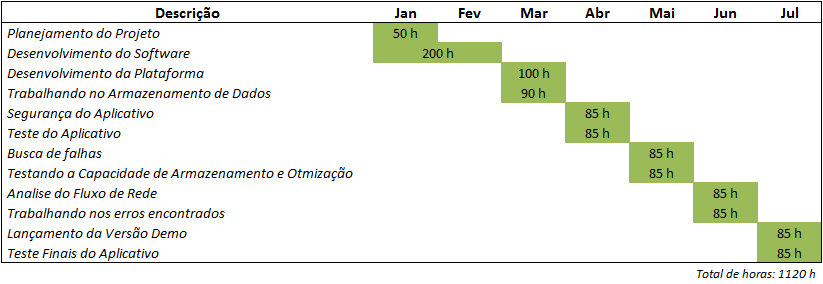
\includegraphics[scale=0.8]{diagramaGanttCrono}
	\end{center}
	%\legend{Fonte: Site da 3GPP}
\end{figure}


% Não está legal. Montar um cronograma \textit{like a} iniciação científica associando o tópico de metas


% Notas de Aula (CICLO DE VIDA)

% Prazos e Tarefas (Inicio, Desenvolvimento e Final) . Fase 1 discussão, planejamento, desenvolvimento planejamento.

% Cada etapa é uma tarefa. Cada tarefa tem um prazo. (HORAS)

%% CICLO
% Levantamento -> Análise - > Projeto -> Implementação -> Manutenção

% Requisito é etapa "Cada momento é um tempo, cada tempo é uma ação" (PROFESSORA)